\documentclass[10pt,a4paper]{scrartcl}
\usepackage[utf8]{inputenc}
\usepackage[english]{babel}
\usepackage{microtype}
\usepackage{amsmath}
\usepackage{mathtools}
%\usepackage[leqno]{amsmath}
\usepackage{amsfonts}
\usepackage{amssymb}
\usepackage{graphicx}
\usepackage{indentfirst}
\usepackage{fancyvrb}
%\usepackage{subfigure}
\usepackage{caption}
\usepackage{subcaption}
\usepackage{enumitem}
\usepackage{booktabs}
\usepackage{algorithm}
\usepackage{algpseudocode}
\usepackage[onehalfspacing]{setspace}
\usepackage[hidelinks]{hyperref}
\usepackage{listings}
\usepackage{xcolor}
\usepackage{fancyhdr}
%\usepackage{tikz}
%\usetikzlibrary{shapes,arrows}
%\pagestyle{fancy}
%\fancyhf{}
%\fancyhead[R]{\thepage}
\usepackage[a4paper,top=3cm,bottom=3cm,left=3cm,right=3cm]{geometry}
\pagenumbering{roman}
% Giuseppe L'Erario

\author{Giuseppe L'Erario}
\date{}
\title{DDPG for cheetah}
\subject{Reinforcement learning}
\begin{document}

\begin{titlepage}
\begin{center}
	
\includegraphics[scale=0.8]{images/SapienzaLogo} \\
	\vspace{3em}
	{\large \textsc{Facoltà di  Ingegneria dell'informazione, Informatica e Statistica}} \\
	\vspace{2em}
%	{\normalsize EE} \\
%	\vspace{1em}
	{\large \textsc{Probabilistic Reasoning and Learning}} \\
	\doublespacing
	\vspace{5em}
	{\Large \textbf{Deep Deterministic Policy Gradient}}
\end{center}

\vskip 2cm
\begin{center}
\begin{tabular}{c c c c c c c c}
	Professor & & & & & & & Student \\[0.2cm]
	\large{Roberto Capobianco} & & & & & & & \large{Giuseppe L'Erario}\\[0.4cm]
\end{tabular}
\end{center}

\vskip 1.5cm
\begin{center}
	{\normalsize Academic Year 2018/2019}
\end{center}
\end{titlepage}

\clearpage{\pagestyle{empty}\cleardoublepage}

\vspace{5em}

\onehalfspacing

\clearpage{\pagestyle{empty}\cleardoublepage}


%\maketitle
\tableofcontents

\clearpage
\pagenumbering{arabic}
\section{Introduction}

Reinforcement learning is a group of algorithms that take as inspiration evolution and learning in the natural world. 

The goal of a typical RL algorithm is to build an agent that learns autonomously how to act in a specific environment on the base of the reward it receives during the process.

\begin{figure}[h]
	\centering
	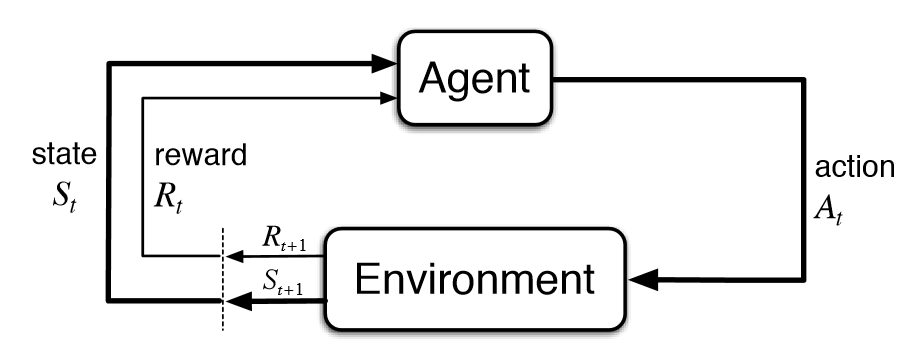
\includegraphics[width=0.7\linewidth]{images/rl}
	\caption{A typical Reinforcement Learning setup.}
	\label{fig:rl}
\end{figure}

Each timestep $ t $ the environment "shows" the actual state to the agent, that takes an action based on its knowledge. This action affects the environment, that returns a new observation and a reward. The reward is then used by the agent as a feedback to update its knowledge.

A great step forward in the field has been made by \textit{DeepMind} in the work \textit{"Continuous control with deep reinforcement learning"} \cite{lillicrap2015continuous}. The core of this paper is one of the most famous RL algorithms: the \textbf{Deep Deterministic Policy Gradient} (DDPG), which will be the subject of this report.

%The report is organized as follows:
%\begin{itemize}
%	\item a brief overview of the state of the art up to the DDPG algorithm;
%	\item a description of the algorithm itself;
%	\item the results obtained by the implemented algorithm on the \texttt{HalfCheetah-v2} environment;
%	\item the evolution of the continuous control RL algorithms after the DDPG.
%\end{itemize}
  
\section{The state of the art up to DDPG algorithm}

As 	previously mentioned, the goal of the Reinforcement Learning is to develop an agent able to improve its performance over time.
 
The behavior of the agent is described by a \textit{policy} function $ \pi:S \rightarrow P(\mathcal{A}) $ that maps the states to a probability distribution over the states. 

An important concept is the \textit{discounted future reward} $ R_t = \sum_{t=i}^{T} \gamma \cdot r(s_i, a_i) = r_t + R_{t+1} $. This quantity represents the reward the agent can gain in the actual state at timestep $ t $ plus the the future rewards that can be obtained acting accordingly to the policy $ \pi $. $ \gamma \in [0,1]$ is the \textit{discount factor} that weights the importance of the future rewards.

The Reinforcement Learning allows agents to automatically learn a policy $ \pi $ that maximizes the discounted future reward $ R $.

Other famous algorithm like \textit{Q-Learning} or \textit{SARSA}\footnote{Respectively, Q-Learning is an OFF-policy algorithm and SARSA an ON-policy one. This means that Q-Learning learns the Q-function based on an action that comes from \textit{another} policy (actually, a greedy policy), while SARSA learns the function based on the \textit{actual} policy of the agent (leading to longer and safer paths w.r.t. Q-learning).} leverage on the concept of the \textit{Q-Value}. It is similar to the discounted future reward $ R $ but takes as input also the action $ a $, describing the future reward $ Q(s,a) $ of the current state $ s $ taking the action $ a $. 

These algorithms work on finite environment. Indeed, Q-learning cannot estimate value for unseen states, restricting its usefulness only to small grid worlds. What if we had possible infinite spaces?

The solution to this problem was found by \textit{DeepMind} (\cite{Mnih2013PlayingAW} and \cite{mnih2015humanlevel}): the \textbf{Deep Q Network} algorithm is capable of overcoming even the humans on many Atari games, a truly breakthrough!

\textbf{DQN} exploits a neural network architecture to estimate the Q-value function. In particular, the neural network takes as input an image representing the actual state and returns as output the estimated Q-value for each action the agent can take.

Prior the DQN, learning using neural networks was difficult and unstable. DQN introduced two innovations that renders stable and robust the learning:
\begin{itemize}
	\item the experience replay;
	\item the target network.
\end{itemize} 

DQN is a valid approach for high-dimensional problems. However, it can face only problems in which only a finite set of discrete actions are available. 

For continuous action spaces one cannot simply discretize the domain: this will lead to the course of dimensionality problem, since thousands of possible actions could originate from a single state. 

Again, \textit{DeepMind} solved this problem by using a neural network architecture to support the \textbf{Deterministic Policy Gradient} algorithm and leveraging on the innovations of \textbf{DQN}.


\section{Deep Deterministic Policy Gradient}

Before describing the DDPG algorithm is useful to recall the concepts of \textbf{Policy Gradient} and \textbf{Q-function}.

While Action-Values methods learn the value of an action, Policy-Gradient methods learn the policy $ \pi(a|s,\theta^\pi) $, that maps the state to the action, stochastic or deterministic\footnote{A stochastic policy tells us that a decision is \textit{likely} to be made. This is useful for exploration of new solutions. A deterministic policy maps \textit{exactly} a state to a precise action.}. 

More specifically, they optimize the \textit{policy function parameters} $ \theta^\pi $ in order to maximize a score function $ J(\theta^\pi) $, clearly related to the reward. This is done in two steps:
\begin{itemize}
	\item measure the quality the policy $ \pi $ using the score function $ J(\theta^\pi) $;
	\item maximize the performance climbing the score function, and hence updating the parameters through gradient ascend: \begin{equation}
		\theta^\pi \leftarrow \theta^\pi +  \alpha \nabla_{\theta^\pi}J(\theta^\pi) \label{update_step}
	\end{equation}
\end{itemize}

The Q-function is computed using the recursive Bellman equation:
\begin{equation}
	Q(s_t,a_t) = \mathbb{E}(r(s_t, a_t) + \gamma Q(s_{t+1}, a_{t+1}))
\end{equation}

\textbf{Deep Deterministic Policy Gradient} relies on an \textit{actor-critic} architecture, meaning that learns approximations of both policy and value functions. More specifically the approximating functions are two neural networks.

The actor learns and uses a \textit{deterministic} policy $ \mu(s,\theta^\mu) $, producing deterministic action based on the current state.

The critic $ Q(s,a,\theta^Q) $ learns how to judge a decision taken by the actor $ \mu(s, \theta^\mu) $ in a given state, relying on the Bellman equation:
\begin{equation}
	y_t = r(s_t, a_t) + \gamma Q (s_{t+1}, \mu(s_{t+1}| \theta^Q))
\end{equation}
and minimizing the loss:
\begin{equation}
	L(\theta^Q) = (Q(s_t,a_t|\theta^Q) - y_t)^2
\end{equation}
and then updating the parameters $ \theta^Q $ in order to approximate the Q-value function.

To update the actor one need to know the expression of the gradient of the score function and then perform the update step \eqref{update_step}.

Silver et al. \cite{silver2014deterministic} provided the expression of the so called \textit{policy gradient}:
\begin{equation}
	\nabla_{\theta^\mu} J = \mathbb{E}[\nabla_{\mu(s_t)}Q(s_t,\mu(s_t)|\theta^Q) \nabla_{\theta^\mu}\mu(s_t|\theta^\mu)]
\end{equation}
that also shows why the policy is deterministic: $ \nabla_{\theta^\mu}\mu(s_t|\theta^\mu) $ cannot be a probability distribution. A deterministic policy, however, is not suitable for exploration. To encourage the discovery of new solutions Ornstein-Uhlenbeck noise is added to the process during the training.

In practice all this is not enough. Neural networks learn correlation between sequential states, despite the problem is structured as a Markov process. This leads to instability. The solution is the same found by the authors of DQN: the \textbf{experience replay}. The algorithm collects experiences in form of tuples $ <s_t, a_t, r_t, s_{t+1}> $ and stores them in a buffer. Then it feeds the networks with a batch of randomly (and so uncorrelated) sampled experiences from the replay buffer.

Furthermore, directly update actor and critic parameters using the gradient leads to divergence. The solution in this case is to create two additional networks, called \textit{target} actor and critic networks, $ \mu{'}(s|\theta^\mu{'}) $ and $ Q{'}(s,a|\theta^Q{'}) $, used to produce the TD error. 

The weights of these target networks $ \theta{'} $are updated slowly using the learned networks weights $ \theta $:
\begin{equation}
	\theta{'} = \tau \theta + (1 - \tau)\theta{'}
\end{equation}
with $ \tau \ll 1 $.

The complete algorithm is shown in fig \ref{fig:algo}.

\begin{figure}[h]
	\centering
	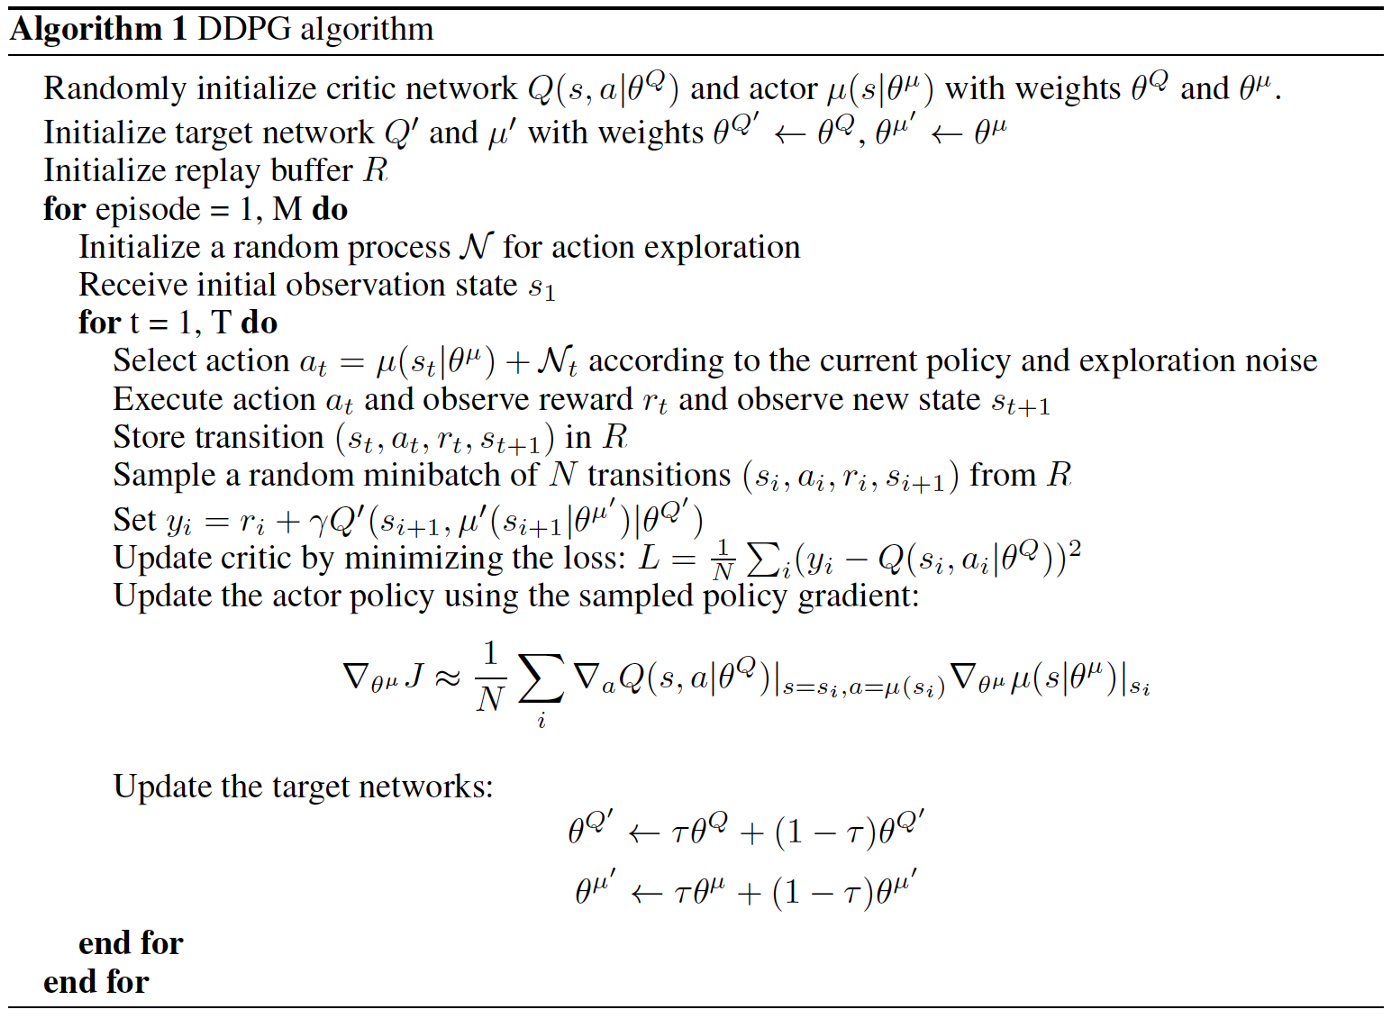
\includegraphics[width=0.8\linewidth]{images/algo}
	\caption{The complete DDPG algorithm.}
	\label{fig:algo}
\end{figure}
 

\section{Results}

\begin{figure}[h]
	\centering
	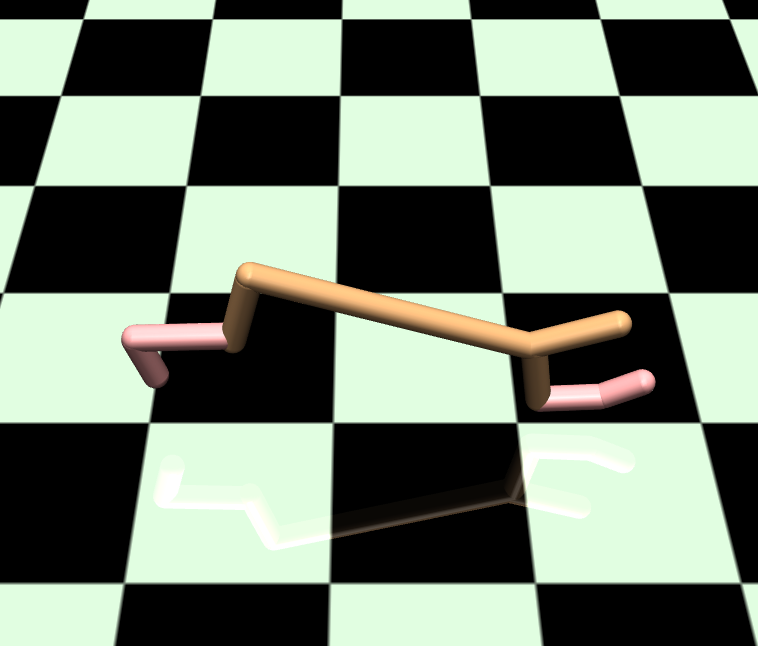
\includegraphics[width=0.5\linewidth]{images/cheetah}
	\caption{The cute half Cheetah.}
	\label{fig:cheetah}
\end{figure}

The implementation is tested on \texttt{HalfCheetah-v2} by \textsc{MuJoCo} using \textsc{Gym}, a toolkit for fast algorithm prototyping developed by \textsc{OpenAi}.

\textsc{Gym} provides the agent with observations and collected reward, relieving the user of the design of the environment.

The \texttt{HalfCheetah-v2} environment has an observation space dimension equal to 17 and an actions space dimension equal to 6. The goal is to let the Cheetah run as much as possible minimizing the control effort.

The chosen parameters for the two networks are those suggested in \cite{lillicrap2015continuous}:
\begin{itemize}
	\item the final output layer of the actor is a \texttt{tanh} to bound the actions. The networks have 2 hidden layers with 400 and 300 units. In the critic network the actions are not included until the second layer.
	\item the learning rate is respectively $ 10^{-4} $ and $ 10^{-3} $ for the actor and the critic, using Adam optimizer;
	\item the soft target update constant $ \tau = 0.001 $;
\end{itemize}

The results are shown in figs \ref{fig:cheetahrew1} and \ref{fig:cheetahrew2}. The training was done in two slots, due to the long training time. After $ \sim 18000 $ episodes and 20 hrs the reward converges to 2700: the Cheetah is able to run!

\begin{figure}[h]
	\centering
	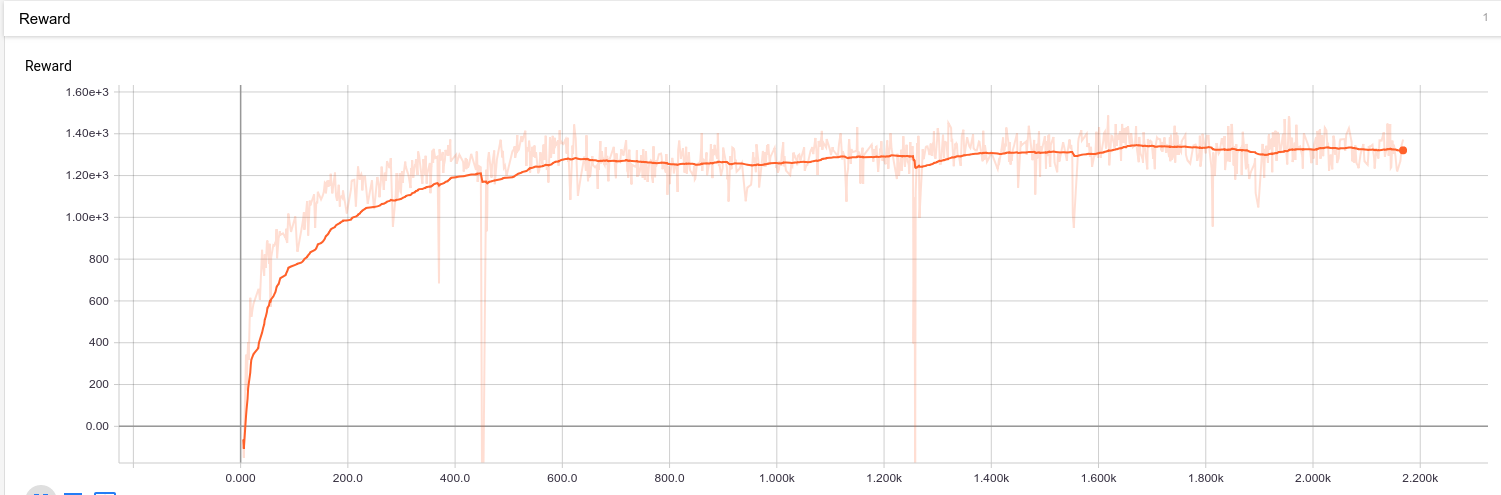
\includegraphics[width=1.0\linewidth]{images/cheetah_rew1}
	\caption{First training slot.}
	\label{fig:cheetahrew1}
\end{figure}
\begin{figure}[h]
	\centering
	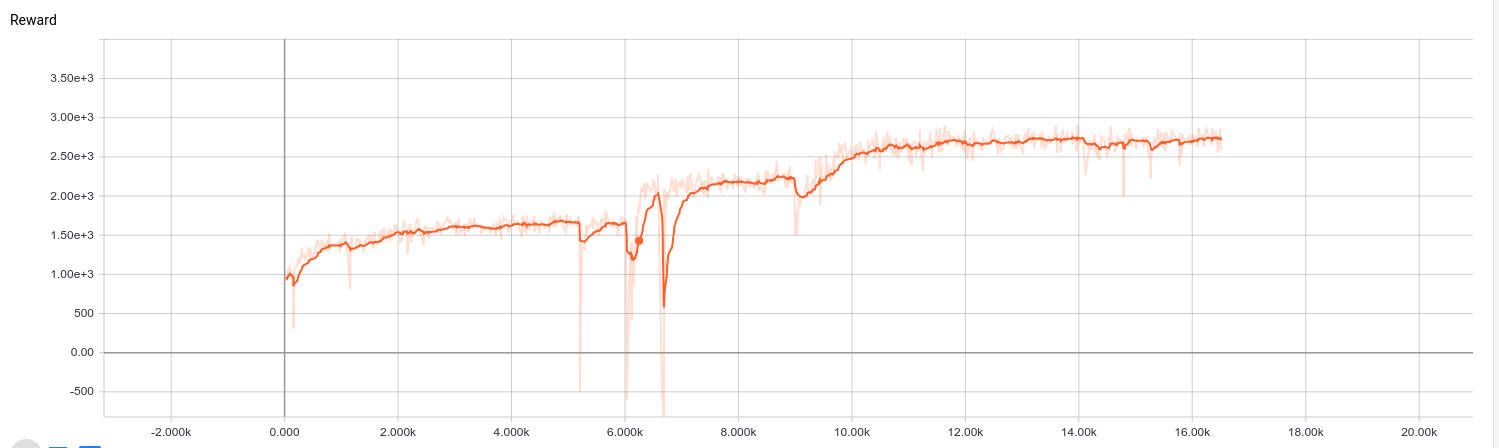
\includegraphics[width=1.0\linewidth]{images/cheetah_rew2}
	\caption{Second training slot.}
	\label{fig:cheetahrew2}
\end{figure}


\section{Conclusions}

As the results show, DDPG is very effective and stable algorithm, despite the use of the neural network.

DDPG is not the state of the art anymore. Nevertheless, it gave birth to a sequence of astonishing continuous control learning algorithm.

For example \textbf{A3C} from \cite{pmlr-v48-mniha16} uses multiple agents that interact with their own instance of the environment. Every agent trains the own network and share the results with the other agents. In this way we do not need the replay buffer and the training is faster. An extension of this algorithm is \textbf{GA3C}, by Nvidia, that uses the GPU.

Still, in policy gradient methods a problem could be how large is the gradient. Indeed  a big step can cause the agent fall off the ``hill''! The authors of \cite{pmlr-v37-schulman15} have found a proper way to restrict the policy change without decreasing the learning rate: \textbf{Trust Region Policy Optimization (TRPO)} speeds the training since the agent walks on a ``very safe path" that leads to the top of the hill.

More recently \textsc{OpenAI} created \textbf{Proximal Policy Optimization (PPO)}: it is based on the same consideration of TRPO but simplifies its formulation.  

\nocite{DDPG_pemami}
\nocite{Simonini}
\nocite{Ben_Lau}



\clearpage

\bibliographystyle{ieeetr}

\bibliography{biblio.bib}
\end{document}
